%%%%%%%%%%%%%%%%%%%%%%%%%%%%%%%%%%%%%%%%%%%%%%%%%%%%%%%%%%%
\section{Theory}
\label{sec:theory}
%%%%%%%%%%%%%%%%%%%%%%%%%%%%%%%%%%%%%%%%%%%%%%%%%%%%%%%%%%%

\begin{algorithm}
\caption{GenerateDesired$x$-spacing($s_1,s_2,e_1,e_2,L$)}\label{alg:XControl}
\begin{algorithmic}[1]
\Require Knowledge of starting $(s_1,s_2)$ and ending $(e_1,e_2)$ positions of  two robots. 
$(0,0)$ is bottom corner, $s_1$ is topmost robot, 
 $L$ is length of the walls. Current position of the robots are $(r_1,r_2)$.
\Ensure   $ r_{1y} - r_{2y}  \equiv s_{1y} - s_{2y} $   %$\Delta y(t) \equiv \Delta y(0)$ 
\State $ \Delta s_x  \gets s_{1x} - s_{2x} $
\State $ \Delta e_x \gets e_{1x} - e_{2x} $
\State $ r_1 \gets s_1$, $ r_2 \gets s_2$
\If {$\Delta e_x < 0 $ }
\State $ m \gets ( L-\max( r_{1x},r_{2x}) ,0)   $ \Comment{Move to right wall}
\Else 
\State  $ m \gets ( -\min( r_{1x},r_{2x}),0 )    $ \Comment{Move to left wall}
\EndIf
\State $m  \gets  m + (0, -\min( r_{1y},r_{2y} ))$ \Comment{Move to bottom}
\State $ r_1 \gets r_1+m$, $ r_2 \gets r_2+m$ \Comment{Apply move}
\If {$\Delta e_x - (r_{1x} - r_{2x} ) > 0 $}
\State $ m \gets (\min(\|\Delta e_x - \Delta s_x \|, L- r_{1x}), 0)$  \Comment{Move right}
\Else
\State $ m \gets (-\min(\|\Delta e_x - \Delta s_x \|, r_{1x}), 0)$\Comment{Move left}
\EndIf 
\State $m  \gets  m + (0, \epsilon)$ \Comment{Move up}
\State $ r_1 \gets r_1+m$, $ r_2 \gets r_2+m$ \Comment{Apply move}
\State $\Delta r_x = r_{1x} - r_{2x}$
\If {$\Delta r_x \equiv \Delta e_x$} 
\State   $ m \gets (e_{1x}-r_{1x}, e_{1y}-r_{1y})$
\State $ r_1 \gets r_1+m$, $ r_2 \gets r_2+m$ \Comment{Apply move}
\State  \Return $(r_1,r_2)$
\Else   
\State \Return GenerateDesired$x$-spacing($r_1,r_2,e_1,e_2,L$)
\EndIf
\end{algorithmic}
\end{algorithm}

\begin{algorithm}
\caption{GenerateDesired$y$-spacing($s_1,s_2,e_1,e_2,L$)}\label{alg:YControl}
\begin{algorithmic}[1]
\Require Knowledge of starting $(s_1,s_2)$ and ending $(e_1,e_2)$ positions of  two robots. 
$(0,0)$ is bottom corner, $s_1$ is rightmost robot, 
 $L$ is length of the walls. Current position of the robots are $(r_1,r_2)$.
\Ensure   $ r_{1x} - r_{2x}  \equiv s_{1x} - s_{2x} $   %$\Delta y(t) \equiv \Delta y(0)$ 
\State $ \Delta s_y  \gets s_{1y} - s_{2y} $
\State $ \Delta e_y \gets e_{1y} - e_{2y} $
\State $ r_1 \gets s_1$, $ r_2 \gets s_2$
\If {$\Delta e_y < 0 $ }
\State $ m \gets ( L-\max( r_{1y},r_{2y}) ,0)   $ \Comment{Move to top wall}
\Else 
\State  $ m \gets ( -\min( r_{1y},r_{2y}),0 )    $ \Comment{Move to bottom wall}
\EndIf
\State $m  \gets  m + (0, -\min( r_{1x},r_{2x} ))$ \Comment{Move to left}
\State $ r_1 \gets r_1+m$, $ r_2 \gets r_2+m$ \Comment{Apply move}
\If {$\Delta e_y - (r_{1y} - r_{2y} ) > 0 $}
\State $ m \gets (\min(\|\Delta e_y - \Delta s_y \|, L- r_{1y}), 0)$  \Comment{Move top}
\Else
\State $ m \gets (-\min(\|\Delta e_y - \Delta s_y \|, r_{1y}), 0)$\Comment{Move bottom}
\EndIf 
\State $m  \gets  m + (0, \epsilon)$ \Comment{Move right}
\State $ r_1 \gets r_1+m$, $ r_2 \gets r_2+m$ \Comment{Apply move}
\State $\Delta r_y = r_{1y} - r_{2y}$
\If {$\Delta r_y \equiv \Delta e_y$} 
\State   $ m \gets (e_{1x}-r_{1x}, e_{1y}-r_{1y})$
\State $ r_1 \gets r_1+m$, $ r_2 \gets r_2+m$ \Comment{Apply move}
\State  \Return $(r_1,r_2)$
\Else   
\State \Return GenerateDesired$y$-spacing($r_1,r_2,e_1,e_2,L$)
\EndIf
\end{algorithmic}
\end{algorithm}

\begin{algorithm}
\caption{WallFrictionArrange2Robots($s_1,s_2,e_1,e_2,L$)}\label{alg:PosControl2Robots}
\begin{algorithmic}[1]
\Require 
Knowledge of starting $(s_1,s_2)$ and ending $(e_1,e_2)$ positions of  two robots. 
$(0,0)$ is bottom corner, $s_1$ is rightmost robot, 
 $L$ is length of the walls. 
 Current position of the robots are $(r_1,r_2)$.
\State $\Delta s_x \gets s_{1x} - s_{2x}$
\State $\Delta s_y \gets s_{1y} - s_{2y}$
\State $\Delta e_x \gets  e_{1x} - e_{2x} $
\State $ \Delta e_y \gets e_{1y} - e_{2y}$
\If {$\Delta s_x < \Delta s_y$}
\State GenerateDesired$x$-spacing($s_1,s_2,e_1,e_2,L$)
\State GenerateDesired$y$-spacing($s_1,s_2,e_1,e_2,L$)
\Else
\State GenerateDesired$y$-spacing($s_1,s_2,e_1,e_2,L$)
\State GenerateDesired$x$-spacing($s_1,s_2,e_1,e_2,L$)
\EndIf

\end{algorithmic}
\end{algorithm}


\begin{figure}
\centering
\begin{overpic}[width = \columnwidth]{Covariance.png}\end{overpic}
\vspace{-1em}
\caption{\label{fig:covFriction} We can control covariance of the swarm by using friction.
}\vspace{-1em}
\end{figure}


\section{Position Control of $n$ robots using wall friction}
Algorithm \ref{alg:PosControl2Robots}  can be extended to control the position of $n$ robots using wall friction under several constraints. Assume an open workspace with four axis-aligned walls with infinite friction.
The axis-aligned rectangle of dimension $(w_f, h_f)$ containing the final configuration of $n$ robots must be disjoint from the axis-aligned rectangle of dimension $(w_s, h_s)$  containing the starting configuration of $n$ robots. Without loss of generality, assume the final configuration is above the starting configuration. 
Furthermore, there must be at least $\epsilon$ space above the final configuration, $\epsilon$ below the starting configuration, and $\epsilon + w_r$ to the left of the final and start configurations, where $w_r$ is the width of a robot.  The workspace is at least $(\epsilon + w_r + \max(w_f,w_s), 2\epsilon + h_s,h_f)$.

Let $(0,0)$ be the lower left corner of the workspace, $p_k$ the $x,y$ position of the $k$th robot, and $f_k$ the final $x,y$ position of the $k$th robot.

\begin{algorithm}
\caption{PositionControl$n$RobotsUsingWallFriction($k$)}\label{alg:PosControl2Robots}
\begin{algorithmic}[1]
\State move( $-\epsilon, -r_{k,y}$) % move  away from right wall and down till robot k touches bottom
\State drift move left until $r_k \equiv (0,0)$
\State drift move up until  $r_{ky} \equiv f_{ky}$

$f_{kx}-f_{(k-1)x}$
$p_{kx}-p_{(k-1)x}$

\State move (  ,0)

\end{algorithmic}
\end{algorithm}


<<<<<<< Updated upstream
\begin{figure}
\begin{center}
%	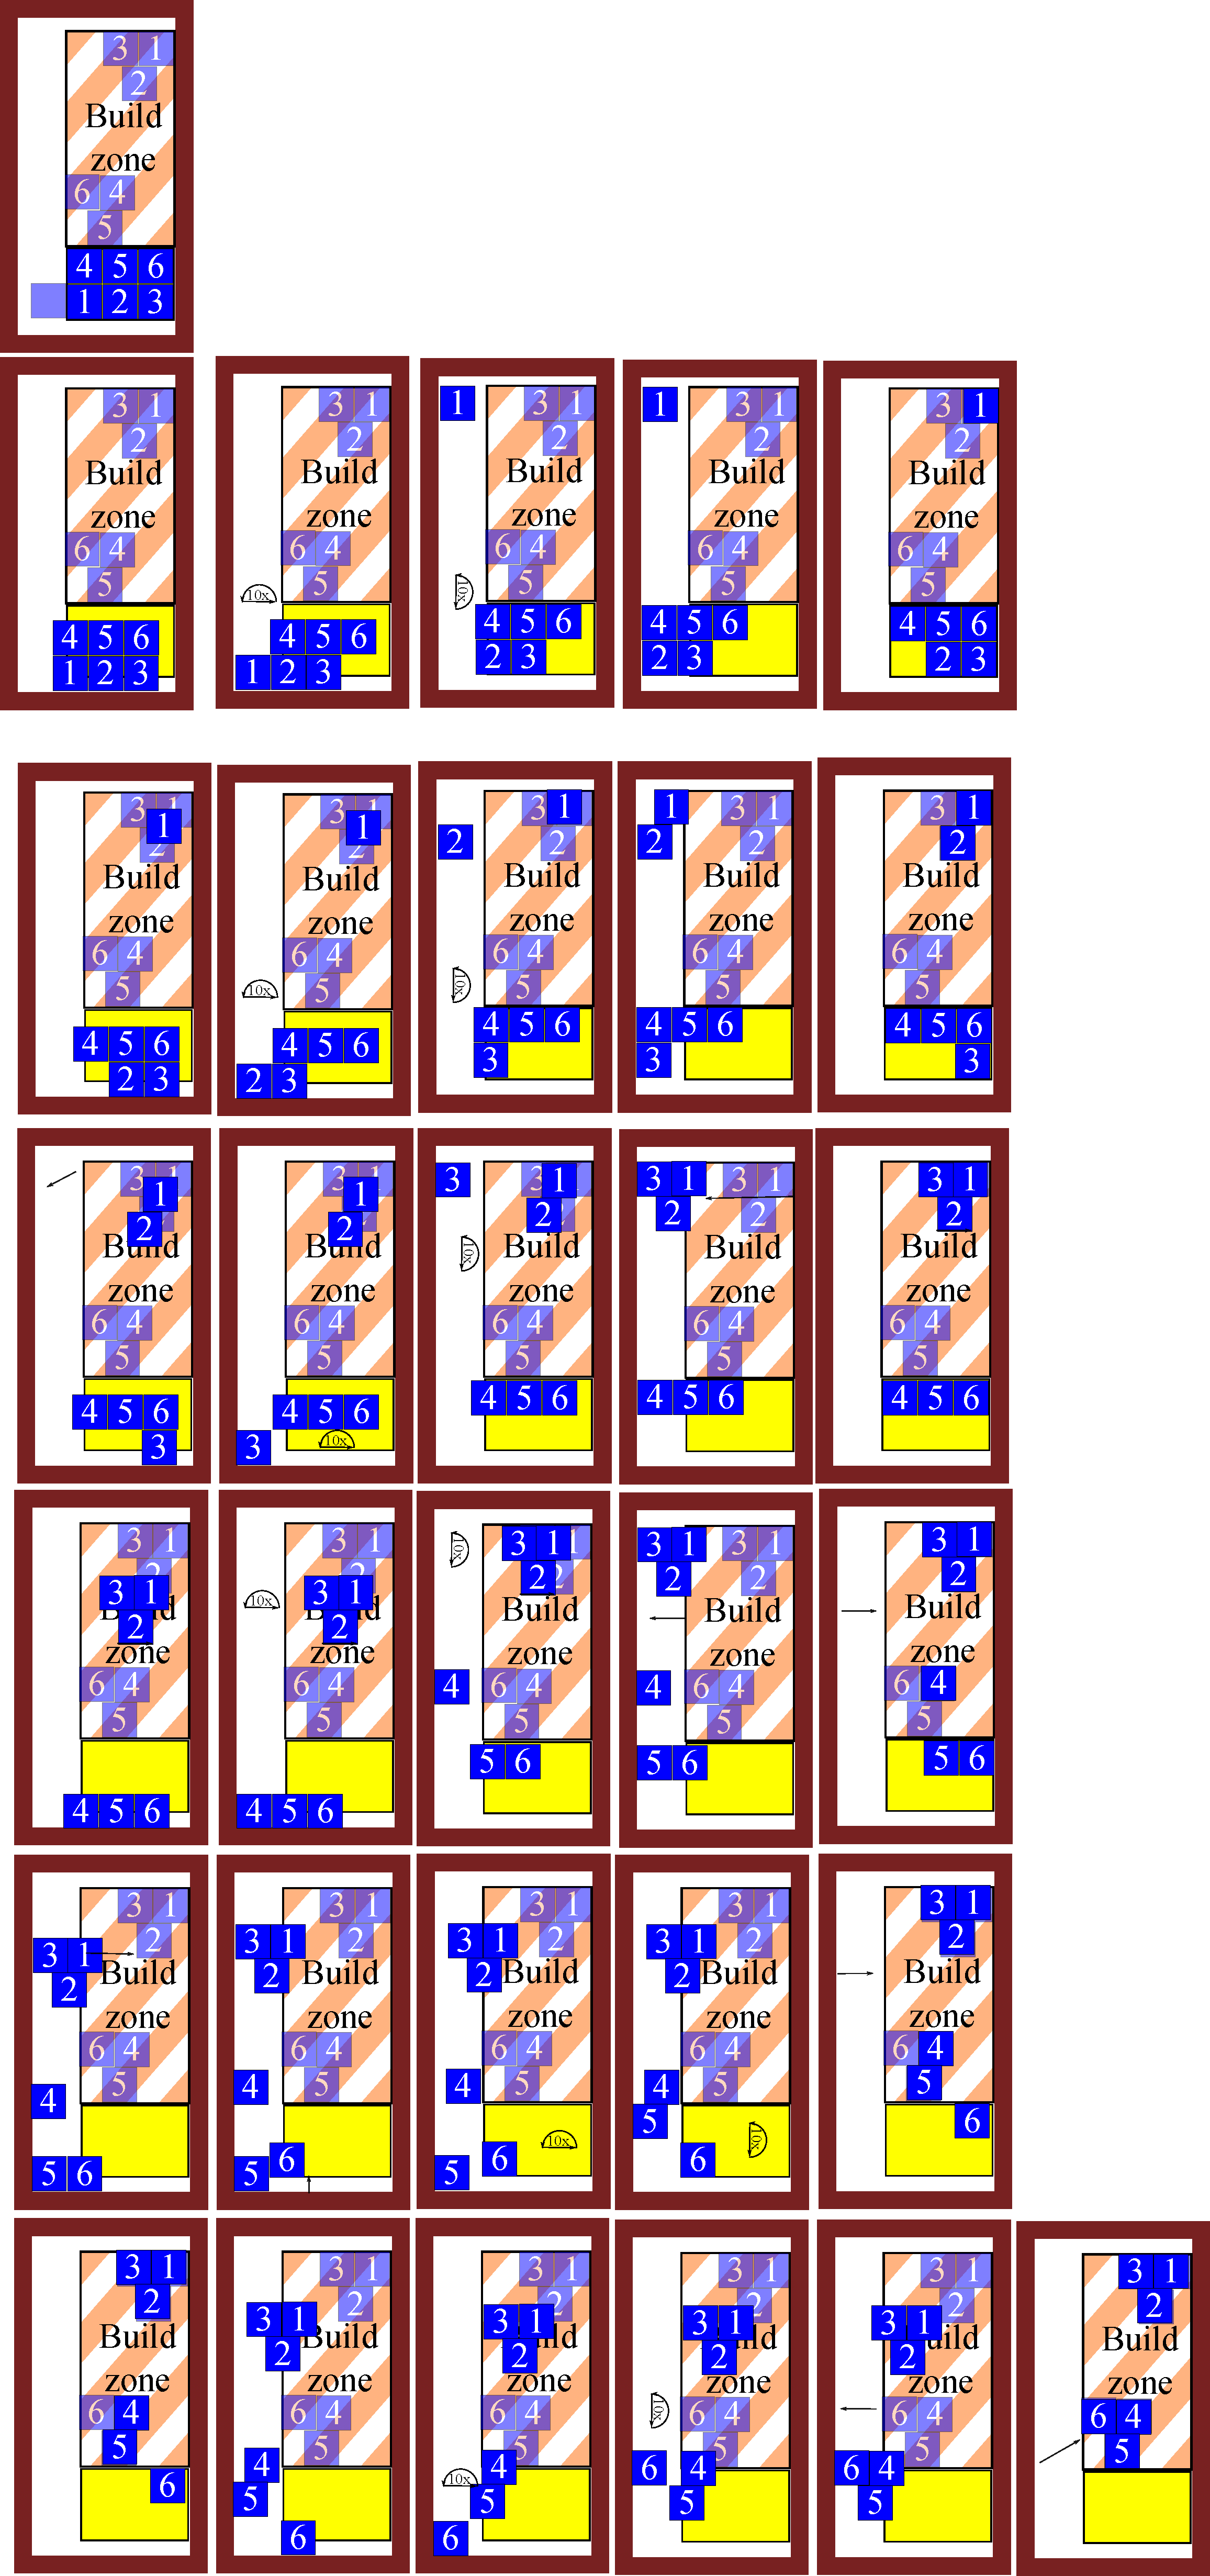
\includegraphics[width=1.0\columnwidth]{construction2dv2.pdf}
\end{center}
\caption{\label{fig:construction2d}
Illustration of algorithm for position control of $n$ robots using wall friction.
}
\end{figure}
=======
%\begin{figure}
%\begin{center}
%	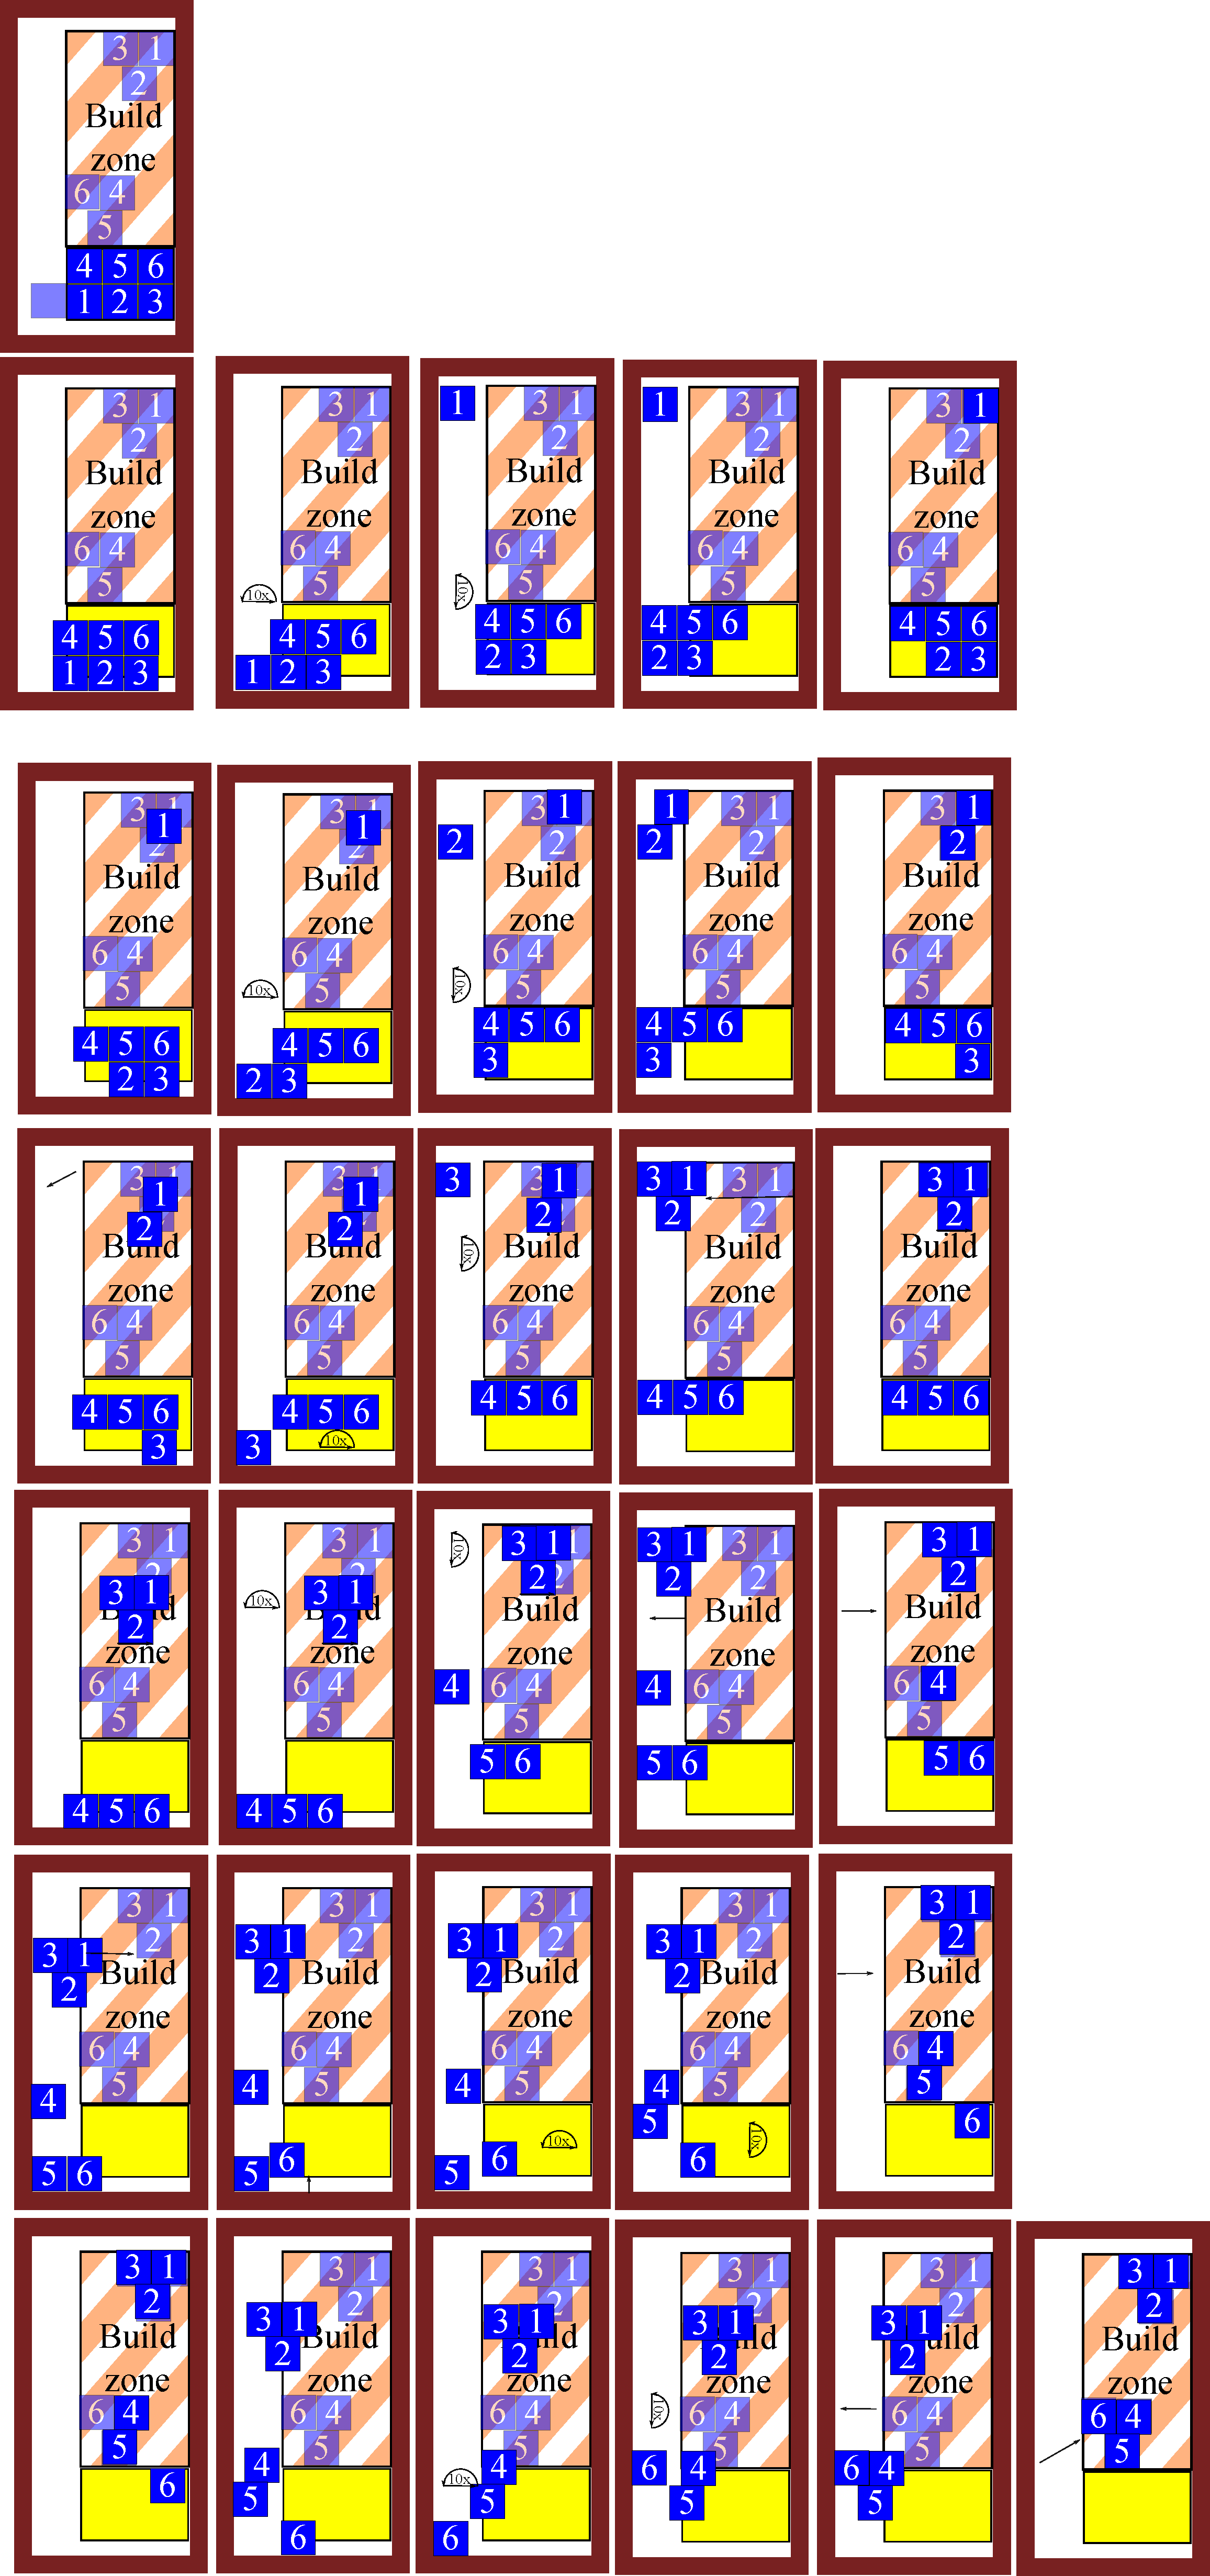
\includegraphics[width=1.0\columnwidth]{construction2dv2.pdf}
%\end{center}
%\caption{\label{fig:construction2d}
%Illustration of algorithm for position control of $n$ robots using wall friction.
%}
%\end{figure}
>>>>>>> Stashed changes




%what images should I show here?
%hysteresis control law, \cite{sadra2014}










